\chapter{Requirement Analysis}
  AutoWDS as it is currently implemented from now on is referred to as AutoWDS basic and the improved system with the features of this requirements analysis realized 
  is called AutoWDS extended.
  Up to now AutoWDS basic automatically uses just one or a random set of channels for its backbone wireless connections. 
  Additionally the topology it creates often reassembles a tree like structure, since the APs connect themselves 
  to the first AP which comes into range and additionally there is no fallback if a link fails. This results not only in huge bottlenecks for throughput,
  it also leads to greater downtimes if a link happens to actually fail. Although the APs automatically rejoin the network if possible, it takes
  a considerable amount of time until they are fully reconnected. This is somehow undesirable for the Systems that use this AP as an uplink connection to
  the network. The following requirements for an improved Version of AutoWDS are supposed to tackle those shortcomings.
  \begin{figure}[t]
    \centering
    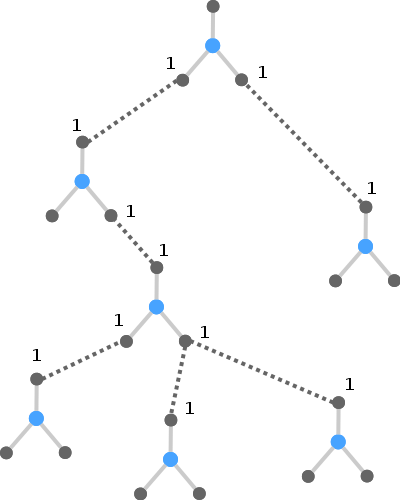
\includegraphics[width=0.3\columnwidth]{figures/autowds_basic_graph}
    \caption{AutoWDS basic network topology and channel assignment}
    \label{fig:autowds_basic_graph}
  \end{figure}
General answer to question of feasibility
  \section{Increase Throughput}
  Since the systems which are connected to the accesspoints consume more data every day and with an increasing storage-footprint of new media like streaming HD videos
  and generally downloading files of up to Gigabytes, a Wireless system is often solely defined by its capability shoveling data over the air to the clients.
  This greed for throughput is amplified by an increasing number of devices that take part in radio communication, 
  thus it is also the key metric for quality in AutoWDS. Furthermore not a single stream of data should be granted exclusively access to the radio, but
  many streams in parallel are desired.
  \section{Reduce Network Connectivity Failures}
  AutoWDS basic is due to its tree like structure very susceptible to connection losses of accesspoints and the infrastructure behind it.
  As this may be just an inconvenience to users of devices like cellphones or laptops who are running non ciritical programs, 
  staying connected in an industrial environment gains in importance where for example heavy machines depend on its uplink connection in order 
  to continue operation. Hence AutoWDS extended shall provide the possibility to create 
  redundant connections in the network topology. The failing scenario is defined as one link breaks while others still being usable.
  \section{Utilize Variable Number of Radios}
  AutoWDS extended will operate with currently up to about 100 accesspoints with a variable amount of radio-modules per accesspoint.
  Current versions of accesspoints are equipped with one up to three radios each. It is supposed to work in heterogenous environment with 
  different numbers of radio-modules per accesspoint. As a consequence the available radio modules 
  have to be utilized as much as possible to achieve gains in overall throughput instead of finding a optimal solution which just uses one radio as this solution is
  still inferior compared to a solution which utilizes multiple radios.
  Switching channels in short intervals to serve more than one channel is explicitly not desired as this leads to packet loss and latency for those channels the radio
  currently not services.
  \section{Capability of Using Variable Channels}
  AutoWDS extended will be used in variable environments and hence may face several restrictions with respect to the channels that are able to be used.
  Thus AutoWDS extended must accept a list of channels only of which it may chose from for channel assignment.
  \section{Restrictions}
    The new solution has to work under the following restrictions:
    \subsection{Centralized Computation}
      AutoWDS extended must also be able to compute its solution on a central entity in contrast to a distributed fashion.
      Also not currently planned, a potential algorithm may be included in the WLC in the future.
      Reconfiguration of accesspoints and collection of data from the accesspoint-network will only be able through a central wireless lan controller.
    \subsection{Static Environment}
      AutoWDS basic and extended is and will be designed for a static environment of accesspoints. That means there will be no highly frequent changes in
      network topology or in link-quality. Although this does not completely render accesspoints immobile, changes if any are expected to be slow and gradually.
\section{Economical Restrictions}
  Neither the central entity nor the accesspoints are limited regarding power consumption. 
  Both will be permanently connected to the power grid and there is no power saving mode which could affect the design or computation.
  AutoWDS extended has to be able to find a solution on demand and in a short timeframe.